%\subsection{Experiment protocol}
Each subject underwent three sessions; one session per day over three consecutive days. The subjects were randomly allocated to either a test or control group; 8 subjects in each group. During each session EMG signals were initially acquired from the subjects and used to train the control system. The subjects then underwent user training with the purpose of learning how to adapt to the control system. Finally the subjects went through a real time performance test to evaluate their ability to operate a virtual prosthesis. In the first session the subject completed the performance test prior to user training. This test was used as a baseline assessment of the subject's performance. All implementations have been performed using MATLAB (2017b). \\
The difference between the test and control groups, and the main area of interest in the study, was in the feedback provided during user training. The test group received the estimated probabilities of each class (confidence scores), while the control group only received label feedback (the estimated class). A flowchart of the study design can be seen in \figref{fig:P:std}.


\begin{figure}[H]                                         
	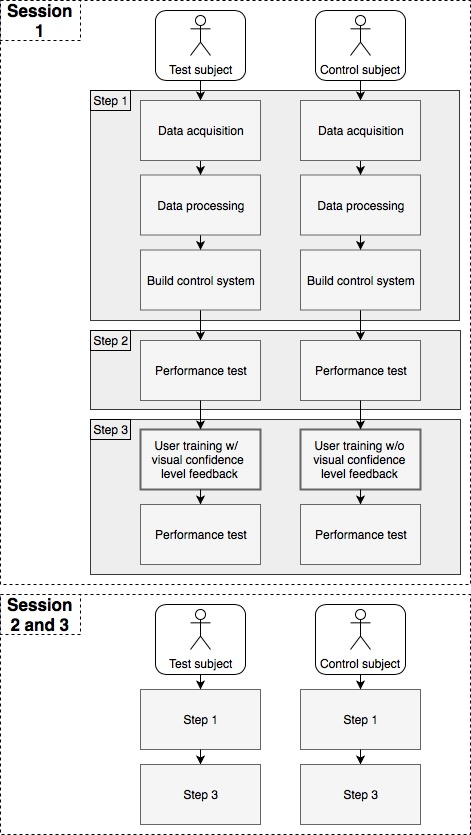
\includegraphics[width=0.42\textwidth]{figures/Paper/Study_design}  
	\caption{Graphical illustration of the experiment showing the steps of each session for the test and control group. Highlighted is user training in step 3 which was the only step that varied between the two groups, and comprised the main area of research interest in the experiment.}
	\label{fig:P:std} 
\end{figure}